\chapter{Write Back}


\begin{figure}
\caption{Write Back}\label{fig:wb}
\begin{center}
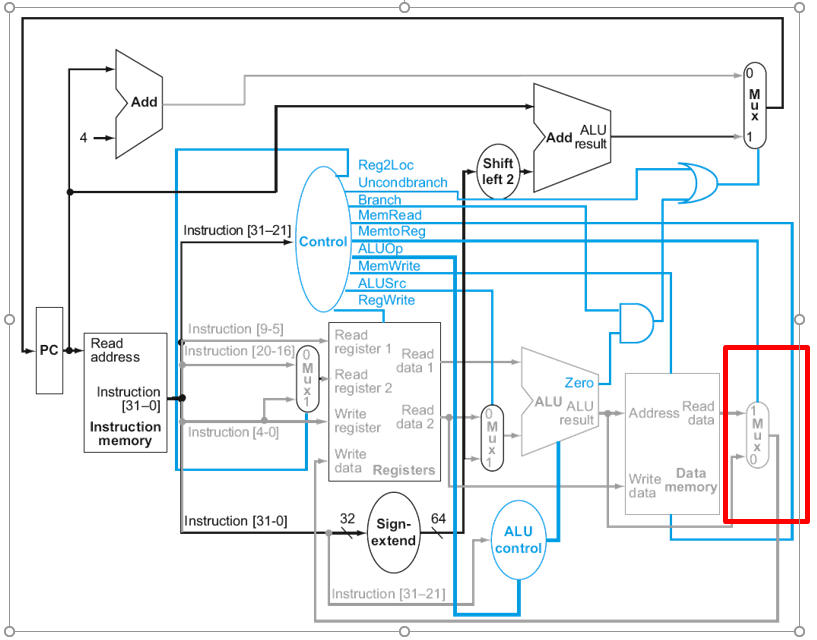
\includegraphics[width=\textwidth]{../images/writeback_stage.png}
\end{center}
\end{figure}

\WrapBarrier

\section{Mux}
This stage consists on only one item, a mux to select between the output of memory and the output of the ALU.  The control is the MemtoReg control line, see Fig~\ref{fig:wb}.  Since the mux has already been tested it does not need a testbench.  The stage thus has only 3 inputs (2 data and 1 control) and one output, the result.

\section{Datapath}
You are ready to assemble the full non-pipelined datapath shown in Fig~\ref{fig:datapath}.  To do this, you will need to combine all 5 stages into datapath.sv.  datapath.sv is a new top-level file, so it is the testbench.  Verify operation of your datapath by running your set of instructions in instrData.data and testing the output.  These instructions are the 10 instructions from the Expected Results Table.  

Now that we have a writeback stage, we do not need to set write\_data in the initial section of datapath.sv.  Rather, you should connect write\_data from the WriteBack stage to the Decode stage.  Because we now have a memory stage, we should no longer need to set pc\_src in the inital section of datapath.sv.  However, our test instructions are not meant to run like a program and would yield strange results.  So for right now, we want to keep pc\_src hard-coded to 0 in datapath.sv.  To do this, we will use a new reg called pc\_src\_tmp and set it to 0.  Then we will use pc\_src\_tmp as the input to the iFetch module.  pc\_src will be a wire that is an output of the iMemory module.  In part 2 of this lab, we will get rid of pc\_src\_tmp and connect pc\_src from iMemory to iFetch.

\begin{figure}
\caption{Full Non-Pipelined Datapath}\label{fig:datapath}
\begin{center}
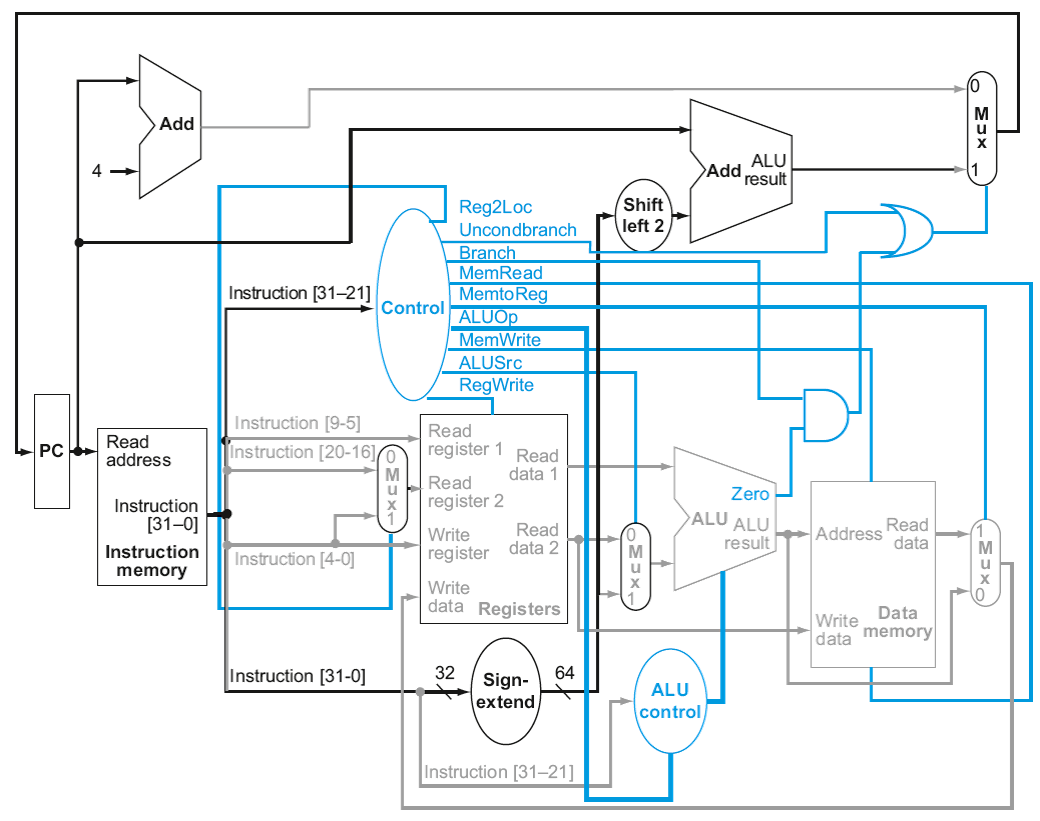
\includegraphics[width=\textwidth]{../images/non_pipelined_datapath.png}
\end{center}
\end{figure}

\section{Your Assignment}

You are to:
\begin{enumerate}
\item Update your Expected Results Table to include the iWriteBack stage.
\item Create the iWriteback stage consisting of one Mux.
\item Integrate all five stages into the file datapath.sv.
\item Run simulations to verify that your results match your Expected Results table.   
	\begin{enumerate}
	\item Your name and the lab number.
	\item A snip of the Simulation Results for both the datapath.sv test and division.sv.  Please show instructions in hex, opcodes and control signals in binary and everything else in signed decimal.  
	\item Copy and paste the entire log for both datapath.sv and division.sv from BEGIN TEST RESULTS to END TEST RESULTS into your file.  The results have gotten too long to use the snipping tool.	
\end{enumerate}
\item Upload Lab11\_lastname.pdf file to Canvas.
\item Zip up your ARM-Lab directory and submit it on Canvas as well.  Please make sure that you give me the ARM-Lab directory rather than the ARM-Project directory.  I do not want the project files in the ARM-Project directory.  Before you submit your zip file, extract the file and make sure that the top-level directory is called ARM-Lab and that the lower level directories like code, manual, etc are directly beneath ARM-Lab in the directory structure.  I will extract your zip file and run your code against my correct testbench to verify that your code and testbench work correctly, and it is critical that everyone's directory structure is consistent.
\end{enumerate} 